\documentclass[10pt, a4paper]{beamer}

\usetheme{Berkeley}
\usecolortheme{sidebartab}

\begin{document}
	\setbeamertemplate{sidebar left}{}
	\title{Progress Presentation-I}
	\subtitle{e-Yantra Summer Intership-2015 \\ PC CONTROLLED TWO WHEEL BALANCE BOT}
	\author{B Suresh\\Ramiz Hussain\\Devendra Kumar Jangir \\ \\ \\
	Mentors: Piyush Manavar,Saurav Shandilya} \\
	\institute{\textbf{IIT Bombay}}
	\date{\today}
	%\addtobeamertemplate{sidebar left}{}{\includegraphics[scale = 0.3]{logowithtext.png}}
	\frame{\titlepage}

\setbeamertemplate{sidebar left}[sidebar theme]
\section{Overview of Project}
\begin{frame}{Overview of Project}
	%$Give following details: \\
	\begin{itemize}
		\item \textbf{Project Name} :PC controlled two wheel balanced bot\\
		\item \textbf{Objective} : To make a two wheel balance bot which can balance itself without any extra support.\\
		\item \textbf{Deliverables}: Two wheeled balanced which can balance itself and move according to the given PC commands.
		\end{itemize}
\end{frame}

\section{Image}
\begin{frame}{Image}
	\begin{figure}
	  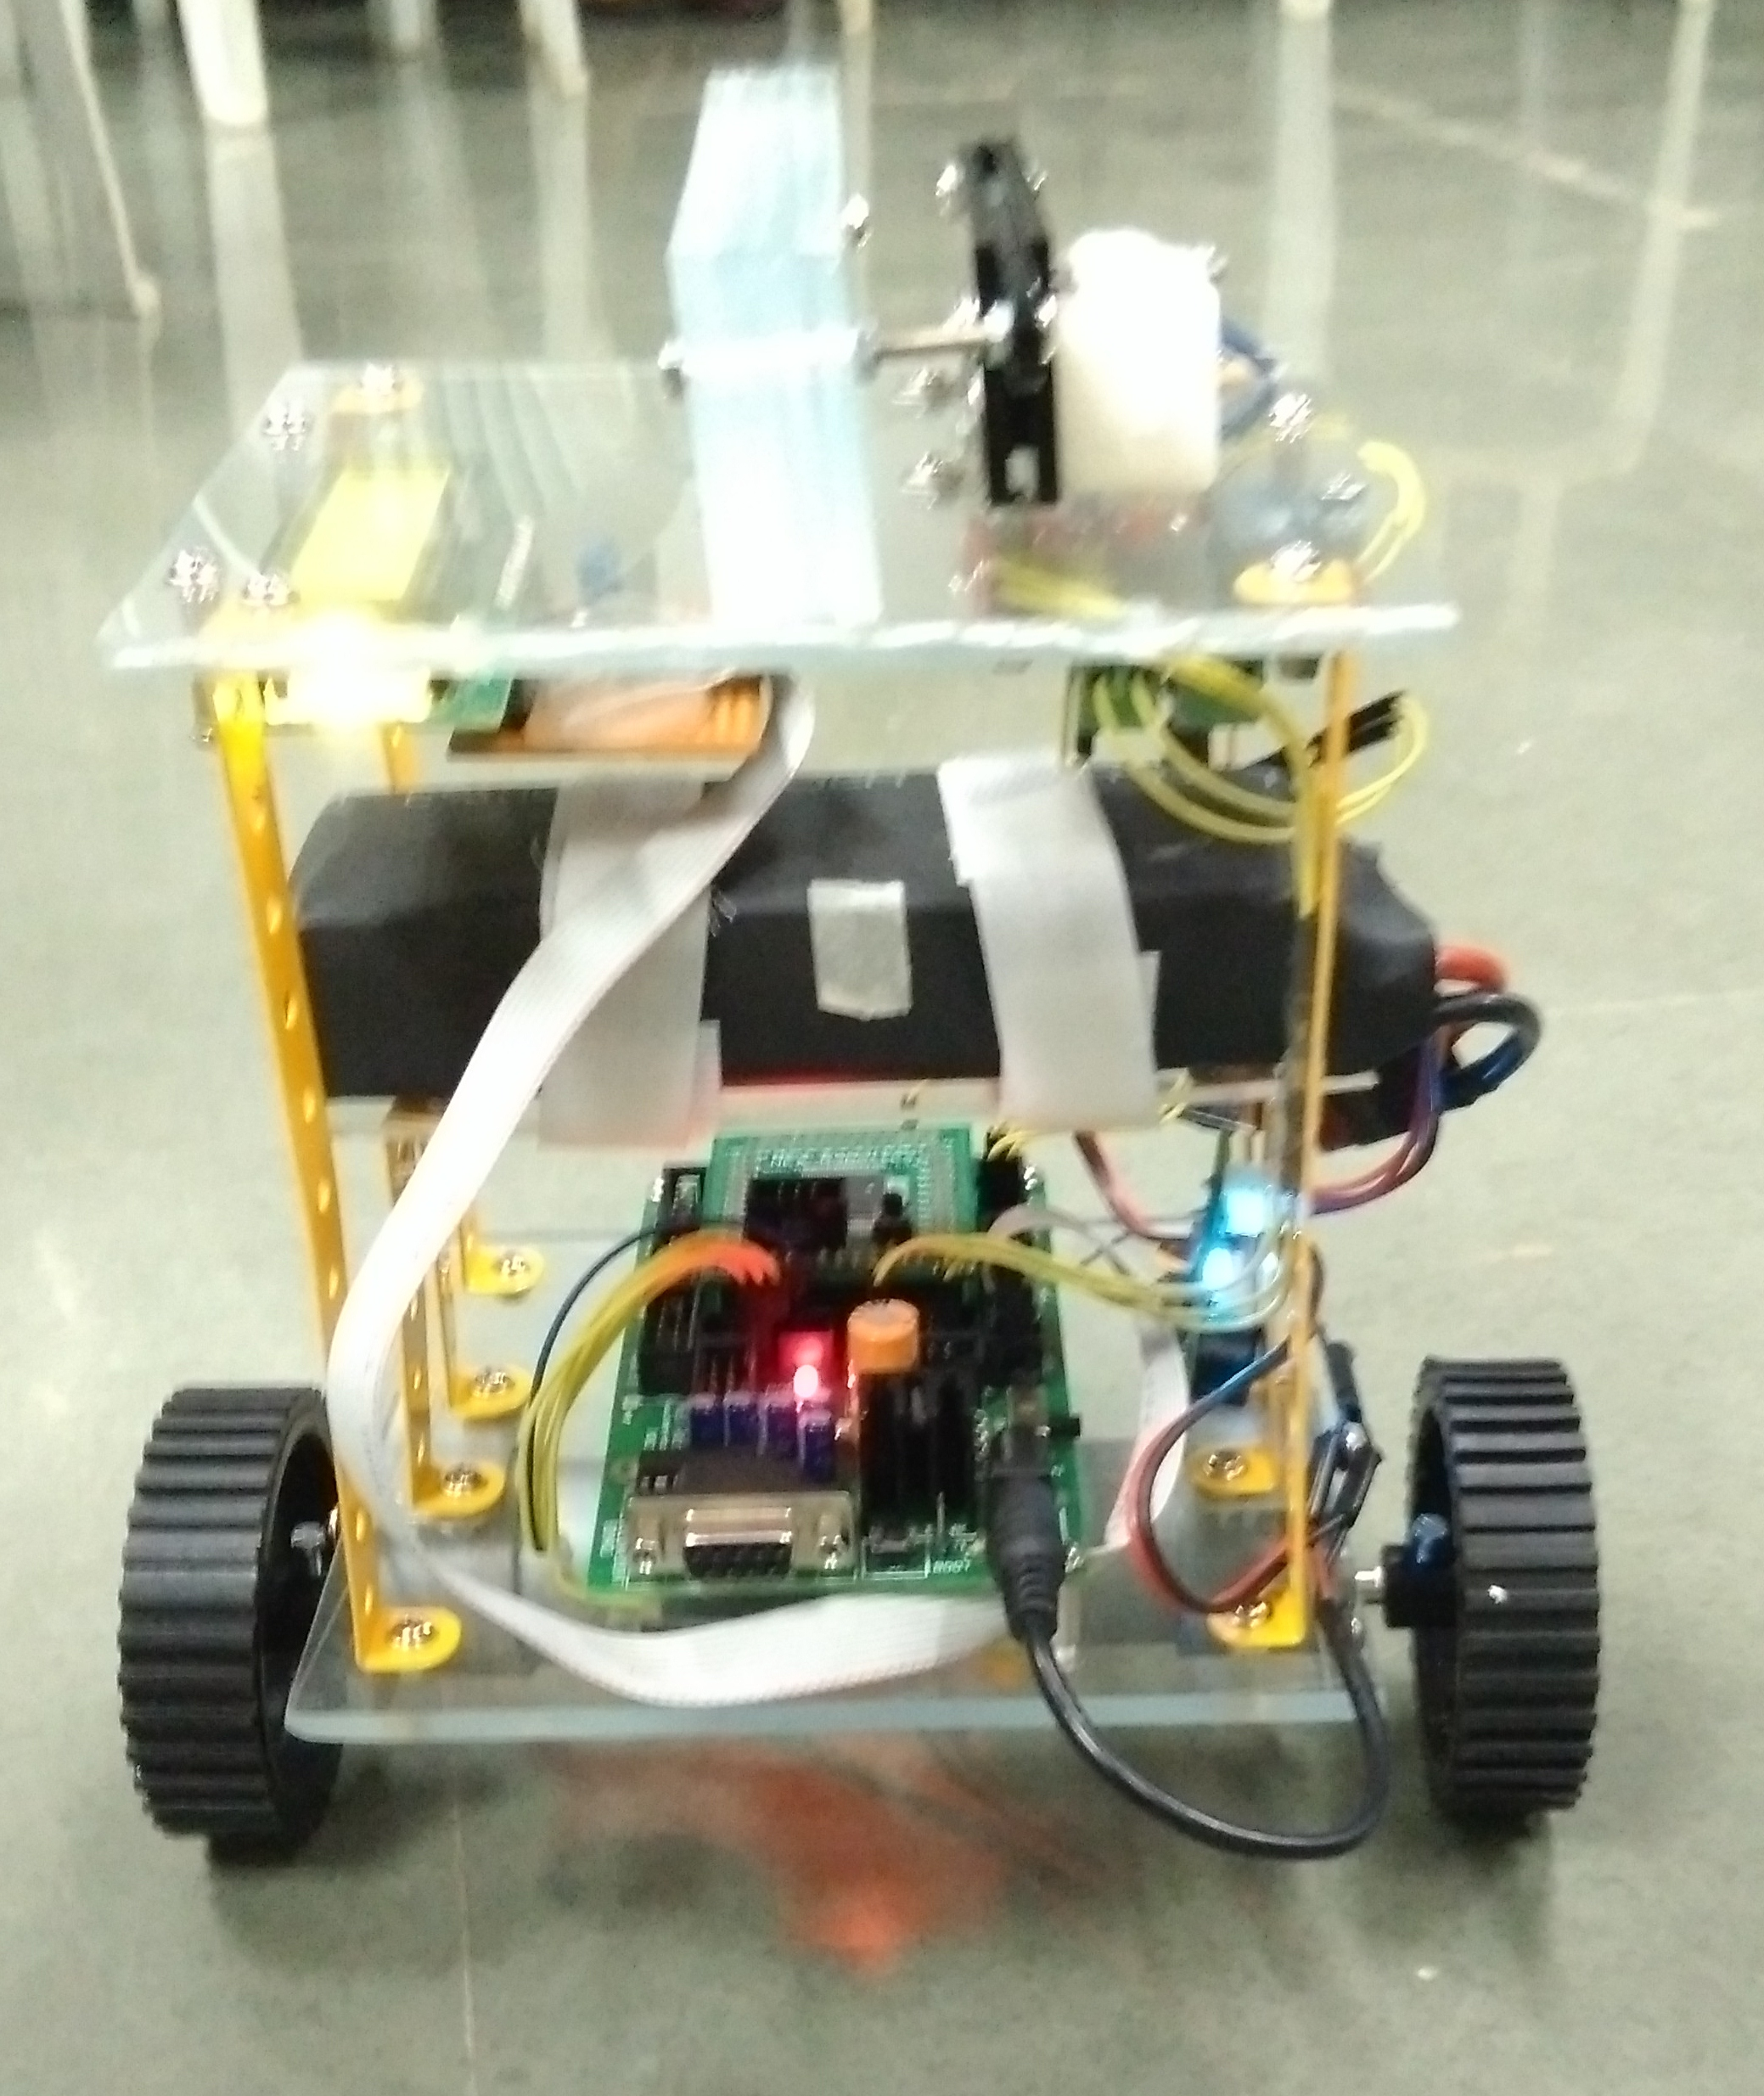
\includegraphics[scale=0.1]{Balance_bot.jpg}
	\end{figure}
\end{frame}

\section{Overview of Task}
\begin{frame}{Overview of Task}
        \begin{enumerate}
		\item Selection of Components,Sensors and Actuators- week 1 \\
		\item Design and fabrication of bot - week 1 \\
		\item Designing of circuit,power management and interfacing - week 1 \\
		\item Algorithm and code implementation for balancing & week 2 and 3 \\
		\item Algorithm and code implementation for locomotion via PC communication & week 4 and 5 \\
		\item Analysis and documentation & week 6 \\
        \end{enumerate}

\end{frame}

\section{Task Accomplised}
\begin{frame}{Task Accomplised}
	\textbf{TASK1:Selection of components,sensors and Actuators} \\
    \begin{enumerate}
     \item DC Motor(300 RPM)
     \item Linear Actuator(150 RPM)
     \item L293D and L298N Motor driver
     \item ATmega 2560 Development board
     \item 16x2 LCD Display
     \item GY-80(Accelerometer and Gyroscope module)
     \item 3 cell Li Po battery 11.1 Volts
     \item Xbee module and adapter
    \end{enumerate}
\end{frame}

\section{Task Accomplished}
\begin{frame}{Task Accomplished}
	\textbf{TASK2:Design and fabrication of bot}\\ \\
	\begin{enumerate}
		\item Fabricating materials
		\item Weight Shifting mechanism
		\item Center of gravity
		\item Protection from falling  
	\end{enumerate}
\end{frame}


\section{Task Accomplished}
\begin{frame}{Task Accomplished}
	\textbf{TASK3:CIRCUIT DESIGN,POWER MANAGEMENT AND INTERFACING}\\ \\
	\begin{enumerate}
		\item L293D and L298N Interfacing
		\item LCD(16x2) 
		\item GY-80(ADXL345 and AGD8) Interfacing  
	\end{enumerate}
\end{frame}


\section{L293D Interfacing}
\begin{frame}{L293D Interfacing}
	\begin{figure}
		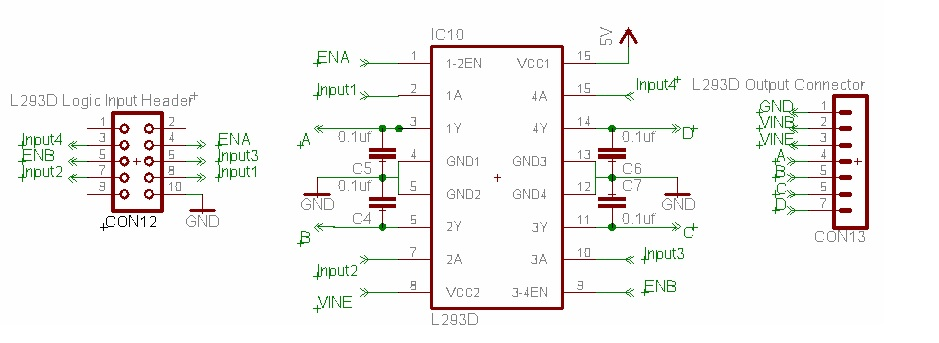
\includegraphics[scale=0.4]{L293d.jpg}
	\end{figure}
\end{frame}

\section{L298N Interfacing}
\begin{frame}{L298N Interfacing}
	\begin{figure}
		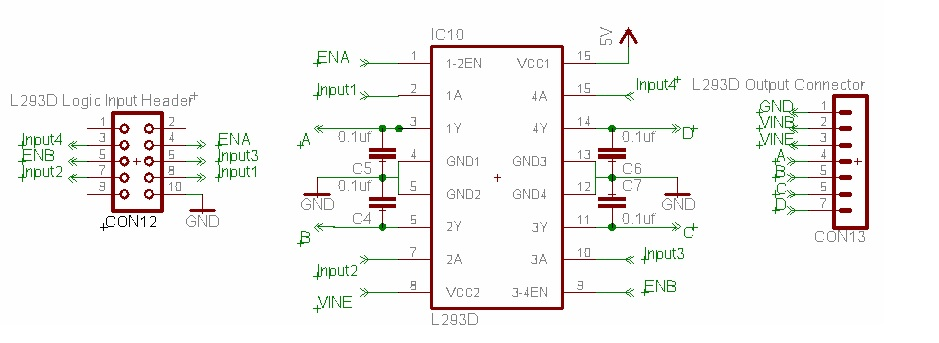
\includegraphics[scale=0.4]{L293d.jpg}
	\end{figure}
\end{frame}

\section{LCD Interfacing}
\begin{frame}{LCD Interfacing}
	\begin{figure}
		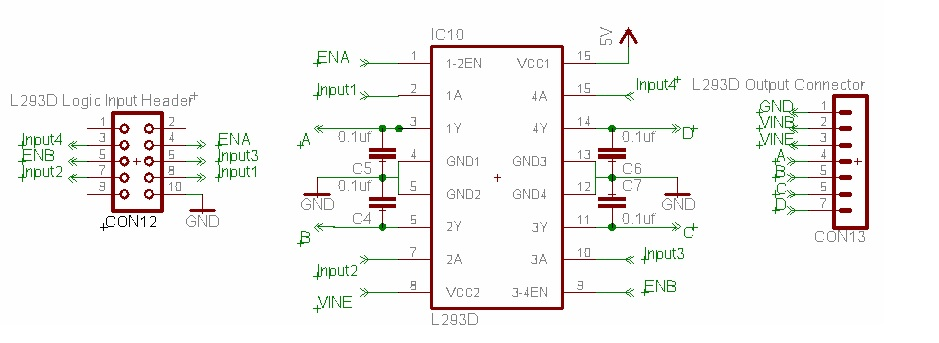
\includegraphics[scale=0.4]{L293d.jpg}
	\end{figure}
\end{frame}



\section{Task Accomplished}
\begin{frame}{Task Accomplished}
	\textbf{TASK4:ALGORITHM AND CODE IMPLEMENTATION}
	\begin{enumerate}
		\item I2C protocol for accelerometer and gyroscope
		\item PWM(10bit Fast PWM or Phase Correct PWM) for controlling velocity of motors 
		\item Timers for PWM and PID calculations
		\item PID Algorithm for balancing the bot 
	\end{enumerate}
\end{frame}


\section{CHALLENGES FACED}
\begin{frame}{CHALLENGES FACED}
	\begin{itemize}
	 \item Maintaining Center Of Gravity(COG) while fabricating the bot
	 \item Understanding and Implementing I2C protocol
	 \item Converting accelerometer values to 10 bit mode and to angles in degrees
	 \item Erroneous reading from accelerometer
	 \item PID tuning  
	 \end{itemize}
\end{frame}

\section{Future Plans}
\begin{frame}{Future Plans}
	\begin{itemize}
		\item PID implementation for balancing and moving the bot
		\item Integrating gyroscope values using Kalman or complementary filter
		\item Xbee interfacing 
	\end{itemize}
\end{frame}


\section{Thank You}
\begin{frame}{Thank You}
	\centering THANK YOU !!!
\end{frame}
\end{document}
